\documentclass[pdftex,12pt,a4paper]{article}
\usepackage[pdftex]{graphicx}
\usepackage{xcolor}
\usepackage{marginnote}
\usepackage{enumitem}
\usepackage[bottom=1.5cm, outer=5cm, inner=2cm, heightrounded,
marginparwidth=4cm, marginparsep=0.5cm]{geometry}

\begin{document}
    % Custom title page
    \begin{titlepage}
        \begin{center}
            
\includegraphics[width=5cm]{figures/kulogo}\\[1cm]
            {\Large \bfseries
                Spring 2014\\
                Computer Networks\\
                CMPE323\\[1cm]
            }
            {\large \bfseries
                \noindent Laboratory Experiment No. 6: Introduction to TCP\\[1cm]
            }
        \end{center}

        \noindent \textbf{Aims and Objectives:}
            \begin{itemize}[leftmargin=4cm]
                \item Introducing Transmission Control Protocol (TCP) and the
                    mechanisms of connection establishment, data transmission,
                    and connection termination.
            \end{itemize}
            \vspace{0.5cm}

        \noindent \textbf{Materials Required:}
            \begin{itemize}[leftmargin=4cm]
                \item IP routers,
                \item Ethernet switches,
                \item PCs with Ethernet adapters,
                \item and straight-through/crossover/rollover cables.
            \end{itemize}
            \vspace{0.5cm}

        \noindent \textbf{Change Log:}
            \begin{itemize}[leftmargin=4cm]
                \item 8-4-2014: original document -- mkhonji.
                \item 9-4-2014: expanded section \ref{howdoestcpwork} with
                    added explanation --
                    mkhonji.
                \item 12-3-2015: fixed a typo -- mkhonji.
                \item 3-2-2016: typo fix in Fig \ref{fig:tcppsh} -- mkhnji.
            \end{itemize}
    \end{titlepage}
    \newpage

    % Lab script content
    \section{Introduction}
        So far, we have covered the following topics:
        \begin{itemize}
            \item \textbf{Layer 1:} Common types of physical mediums that
                allow the transmission of bits to and from connected nodes.
                This was achieved in the lab via twisted-pairs of copper wires
                using Cat6e cables and RJ45 connectors. We've also explored how
                RX and TX pins can be connected accordingly via cross-over and
                straight-through cables, as well as Auto-MDIX for automatic pin
                re-arrangement within Ethernet network adapters.

            \item \textbf{Layer 2:} Broadcast domains (e.g. Ethernet),
                scalability issues that we face if the broadcast domains grow
                too large, and how to reduce their size.  This was achieved by
                physical separation as well as logical separation of broadcast
                domains using VLANs and IEEE 802.1Q tags over trunking ports.

            \item \textbf{Layer 3:} A scalable architecture that allows nodes
                within \emph{different} broadcast domains to communicate with
                each other. This introduced IP and CIDR which allowed
                end-to-end reachability.

            \item \textbf{Layer 4:} A mechanism by which applications on nodes
                can specify not only which destination node they wish to
                communicate to, but also specify which application or service
                they wish to receive the sent messages. So far, we have only
                covered UDP --- a simple minimalist protocol that does just
                that.
        \end{itemize}

        In this lab, we will study another \emph{layer 4} protocol, namely:
        Transmission Control Protocol (TCP). However, before we describe what
        TCP is, let's first see the advantages and the disadvantages of UDP.

        \subsection{Why is UDP good?}
            Before we look at the limitations of UDP, it is important to note
            that, due to the simplicity of UDP, it is a pretty good choice for
            scenarios where low-delay transmission of data is needed. 
            
            For example, if you are playing some multi-player first-person
            shooter game over the network and that you press the trigger to
            fire a bullet towards some moving object (e.g. running enemy
            vehicle).
            
            In the example above, it is very important to ensure that the
            message (that signals the firing of the bullet to the server) is
            sent as soon as possible to the server. If there is any
            transmission delay, then by the time the message is delivered to
            the server, the object may have moved too far away.

            This is why time-sensitive applications use UDP. This includes
            applications such as the Domain Name System (DNS) where
            transmission delay can cause significant effects against the
            overall end-user experience.

        \subsection{Why is UDP not enough?}
            UDP does not provide the following by itself:
            \begin{itemize}
                \item \textbf{Reliable data transmission:} e.g. when sender $S$ sends
                    packet $P$ to receiver $R$, and if $P$ was dropped along
                    the path before it reached $R$, then UDP does not provide
                    (by itself) any mechanism to identify such packet loss and
                    thus $P$ will not be retransmitted by UDP.
                \item \textbf{Ordered data delivery:} UDP does not provide
                    any mechanism by itself by which the receiver can ensure
                    that the order of reception is the same as the order of
                    transmission. In other words, if the sender $S$ sent packets
                    $(P_1, P_2)$ in this order to some receiver $R$, and if
                    $R$ received the packets in a different order $(P_2, P_1)$,
                    then UDP provides no mechanism by itself for $R$ to
                    identify the correct order.
                    
                \item \textbf{Flow control:} e.g. when sender $S$ sends some packet $P$
                    to receiver $R$, then there is no mechanism that is
                    provided by UDP itself to let $S$ know how much data $R$ is
                    able to receive/process. This way, $S$ may overwhelm $R$
                    with excessive amounts of data and yet $S$ does not know
                    that $R$ is under too much load.
                \item \textbf{Congestion control:} e.g. when some network congestion
                    accrues, there is no mechanism that is provided by UDP to
                    automatically reduce the transmission rate in order to
                    reduce the congestion.
            \end{itemize}

            However, it is important to note that while UDP does not provide
            the above mechanisms by itself, there is nothing that forbids UDP
            applications to implement their own application-layer mechanisms
            that facilitate the above. For example, a UDP application may
            implement reliable data transmission in its application layer by
            sending acknowledgements of received data.

        \subsection{Why do we need TCP?}
            There are many applications that require reliable data
            transmission, flow control and congestion control, while (at the
            same time) are not delay-sensitive. Examples are HTTP, FTP, SMTP,
            IMAP, POP3, Telnet, SSH, \ldots. Since there are many applications
            that require such features, then having each application implement
            its own set of mechanisms is redundant and time-consuming.

            Due to the reason above, it is clear that it would be useful if a
            layer 4 protocol provided the above mechanisms by itself, so that
            all application layer protocols can \emph{transparently} take
            advantage of them without the need of coding them into their
            application layer.

            This is exactly what TCP does: a layer 4 protocol that provides the
            following additional mechanisms: reliable data transmission,
            ordered data delivery, flow control, congestion control. UDP
            provides error detection and so does TCP. Therefore, if your
            application is not delay-sensitive and needs the mechanisms above,
            then TCP is a good choice.

        \subsection{How does TCP work?}\label{howdoestcpwork}
            In this lab, we will cover the basic behaviour of TCP, which is a
            subset of what is defined in RFC793. 

            However, it should be noted that changes beyond RFC793 exist. This
            is due to a number of reasons, one of which is that TCP allows for
            extensions via variable length options, as well as the existence of
            tweakable parameters in TCP's operation (e.g. multiple timer
            parameters and finding the right timers is a an open optimization
            problem. For example, RFC7298 was proposed as late as 2011 to
            present a newer method for calculating the re-transmission timer).

            Simply put, the most visible principles of TCP that achieve that
            are:
            \begin{itemize}
                \item Use of sequence numbers: all transmitted data are given
                    sequence numbers that receivers must acknowledge by
                    sending back the incremented sequence number by one.
                    I.e. if node $R$ receives an octet with the sequence number
                    \texttt{SEQ} = 1, then $R$ must acknowledge it by sending an
                    acknowledgement number \texttt{ACK} = \texttt{SEQ} + 1 =
                    1+1 = 2 back to the sender $S$.
                \item Use of timers: if an acknowledgement is not received
                    within some time interval, then actions will be taken
                    accordingly. For example, if the sender node $S$ sent some
                    data to the receiver node $R$ and $S$ did not receive any
                    acknowledgements back from $R$ for some time $T$, then $S$
                    will assume that the data was lost will then retransmit it
                    again. Additionally, $R$ will also slow-down its
                    transmission speed (by reducing its transmission window
                    size) in an attempt to avoid possible causes of the assumed
                    data loss (e.g. network congestion, or if $R$ was too busy
                    processing previous data).
            \end{itemize}

            In this lab, we will focus on: connection establishment, data
            transmission, and connection termination.

            \subsubsection{Connection establishment}
                TCP requires that, prior to the transmission of any data, a
                connection to be established first. Such connection
                establishment happens via what's known as \emph{TCP's 3-way
                hand-shake}. The goal of this stage is simple: identifying the
                sequence number the first bytes of both of the communicating peers.

                An example is depicted in Figure \ref{fig:tcpsyn} by which
                the peers A and B agreed at sequence numbers 101 and 301
                respectively.

                \begin{figure}[tbh]
                        \centering
                        \small\begin{verbatim}   TCP A                                                TCP B
1. CLOSED                                               LISTEN
2. SYN-SENT    --> <SEQ=100><CTL=SYN>               --> SYN-RECEIVED
3. ESTABLISHED <-- <SEQ=300><ACK=101><CTL=SYN,ACK>  <-- SYN-RECEIVED
4. ESTABLISHED --> <SEQ=101><ACK=301><CTL=ACK>      --> ESTABLISHED\end{verbatim}\normalsize
                \vspace{-15pt}
                \caption{TCP's three-way hand-shake for connection
                establishment --- Source RFC793.}
                \label{fig:tcpsyn}
                \end{figure}

            \subsubsection{Data transmission}
                Once the TCP 3-way hand-shake is successfully performed to
                obtain the sequence numbers, it is possible for the involved
                peers to transmit data as depicted in Figure \ref{fig:tcppsh}.
                Notice how the transmitted data ``\texttt{Hello}'' is composed
                of 5 octets with its first octet having the sequence 101, which
                resulted in the peer B to acknowledge its  reception by sending
                an acknowledgement of 101 + 5 = 106. In other words, the
                acknowledgement is the sequence number of the first octet +
                the total number of received octets since the first one.

                \begin{figure}[tbh]
                        \centering
                        \small\begin{verbatim}   TCP A                                                   TCP B
1. ESTABLISHED --> <SEQ=101><ACK=301><CTL=PSH><Hello>  --> ESTABLISHED
2. ESTABLISHED <-- <SEQ=301><ACK=106><CTL=ACK>         <-- ESTABLISHED\end{verbatim}\normalsize
                \vspace{-15pt}
                \caption{TCP's data communication.}
                \label{fig:tcppsh}
                \end{figure}

            \subsubsection{Connection termination}
                Similar to the connection establishment, except for using the
                \texttt{FIN} flag instead of the \texttt{SYN} flag. As depicted
                in Figure \ref{fig:tcpfin}, note how the sequence numbers are
                continuations of the last sequence numbers.

                \begin{figure}[tbh]
                        \centering
                        \small\begin{verbatim}   TCP A                                                TCP B
1. ESTABLISHED                                          ESTABLISHED
2. FIN-WAIT    --> <SEQ=106><CTL=FIN>               --> CLOSE-WAIT  
3. TIME-WAIT   <-- <SEQ=301><ACK=107><CTL=FIN,ACK>  <-- LAST-ACK    
4. CLOSED      --> <SEQ=107><ACK=302><CTL=ACK>      --> CLOSED\end{verbatim}\normalsize
                \vspace{-15pt}
                \caption{TCP's three-way hand-shake for connection termination.
                    Note that this is a simplification for the original 4-way
                    hand-shake that is described in RF793. I.e. instead of
                    having peer \texttt{B} send two TCP packets (one packet
                    \texttt{ACK}ing peer A's \texttt{FIN} and another indicating
                    its own desire by terminate the connection by setting the
                    \texttt{FIN} flag), it combines them in a single packet (one
                    packet that has both \texttt{ACK} and \texttt{FIN} flags set.}
                    \label{fig:tcpfin}
                \end{figure}

            \subsubsection{Header format}
                \begin{figure}[tbh]
                        \centering
                        \small\begin{verbatim} 0                   1                   2                   3
 0 1 2 3 4 5 6 7 8 9 0 1 2 3 4 5 6 7 8 9 0 1 2 3 4 5 6 7 8 9 0 1
+-+-+-+-+-+-+-+-+-+-+-+-+-+-+-+-+-+-+-+-+-+-+-+-+-+-+-+-+-+-+-+-+
|          Source Port          |       Destination Port        |
+-+-+-+-+-+-+-+-+-+-+-+-+-+-+-+-+-+-+-+-+-+-+-+-+-+-+-+-+-+-+-+-+
|                        Sequence Number                        |
+-+-+-+-+-+-+-+-+-+-+-+-+-+-+-+-+-+-+-+-+-+-+-+-+-+-+-+-+-+-+-+-+
|                    Acknowledgment Number                      |
+-+-+-+-+-+-+-+-+-+-+-+-+-+-+-+-+-+-+-+-+-+-+-+-+-+-+-+-+-+-+-+-+
|  Data |           |U|A|P|R|S|F|                               |
| Offset| Reserved  |R|C|S|S|Y|I|            Window             |
|       |           |G|K|H|T|N|N|                               |
+-+-+-+-+-+-+-+-+-+-+-+-+-+-+-+-+-+-+-+-+-+-+-+-+-+-+-+-+-+-+-+-+
|           Checksum            |         Urgent Pointer        |
+-+-+-+-+-+-+-+-+-+-+-+-+-+-+-+-+-+-+-+-+-+-+-+-+-+-+-+-+-+-+-+-+
|                    Options                    |    Padding    |
+-+-+-+-+-+-+-+-+-+-+-+-+-+-+-+-+-+-+-+-+-+-+-+-+-+-+-+-+-+-+-+-+
|                             data                              |
+-+-+-+-+-+-+-+-+-+-+-+-+-+-+-+-+-+-+-+-+-+-+-+-+-+-+-+-+-+-+-+-+\end{verbatim}\normalsize
                \vspace{-15pt}
                \caption{TCP's header format --- Source RFC793.}
                \label{fig:tcp}
                \end{figure}

                TCP's fields are (fields that are beyond the scope are marked as
                gray):
                \begin{itemize}
                    \item Source and destination port numbers: each is 16 bits.
                    \item Sequence and acknowledgement numbers: each is 32bits.
                    \item Data offset: this is essentially TCP's header length in units
                        of 32bits. Thus the minimal size is 5 (assuming no option
                        fields are used).
                    \item Future reserved bits: 5 bits that are not used according
                        to RFC793, however, later RFCs that are beyond the scope of
                        this lab have proposed methods to utilize those reserved
                        bits.
                    \item Flags: 6 on/off flags (each is 1 bit). The flags that are
                        covered in this lab are ACK, PSH, SYN and FIN.
                    \item Window: 16 bits that indicate receivers buffer. The unit
                        is in octets by default (however, TCP allows for changing
                        the unit via the use of TCP option headers, which is beyond
                        the scope of this lab).
                    \item Checksum: 16 bits of one's complement of one's complement
                        sum of all 16 bit words of the TCP header, payload and the pseudo IP header
                        as depicted in Figure \ref{fig:tcpsip}.
                    \item {\color{gray}Urgent pointer: 16 bits number that indicates an offset
                        from the current byte sequence down to some byte
                        sequence. Bytes that fall within this range are considered
                        urgent and will be processed first by the receiver
                        (beyond the scope of the lab).}
                    \item {\color{gray} Options: variable length, used to extend TCP (beyond the
                        scope of this lab).}
                    \item Data: variable length sequence of bits to accommodate
                        user data.
                \end{itemize}

                \begin{figure}[tbh]
                    \centering
                        \small\begin{verbatim}                +--------+--------+--------+--------+
                |           Source Address          |
                +--------+--------+--------+--------+
                |         Destination Address       |
                +--------+--------+--------+--------+
                |  zero  |  PTCL  |    TCP Length   |
                +--------+--------+--------+--------+\end{verbatim}\normalsize
                    \vspace{-15pt}
                    \caption{Pseudo IP header format as used in TCP's checksum
                    calculation, where \texttt{PTCL} is protocol ID --- Source RFC793.}
                    \label{fig:tcpsip}
                \end{figure}

    \section{Lab Preparation}
        \begin{enumerate}
            \item Connect a PC to the routers console port using a rollover
                cable\footnote{If using Linux: \texttt{screen /dev/ttySx} were
                \texttt{x} is the
                serial interfaces ID that is connected to the console
                cable. If using Windows: Use Hyperterminal or Putty to
                connect to \texttt{COMx} ports.}.
            \item Erase the configuration of the
                routers\footnote{\texttt{enable}, \texttt{erase
                startup-config}, \texttt{reload}, and make sure to answer
                \texttt{no} to all yes/no questions while hitting
                \emph{enter} for all \texttt{confirm} prompts.}.
            \item Connect a PC to the switches console ports using rollover
                cables.
            \item Erase the configuration of the
                switch\footnote{\texttt{enable}, \texttt{erase startup-config},
                \texttt{delete vlan.dat}, \texttt{reload}, and answer
                \texttt{no} to all yes/no questions while hitting
                \emph{enter} for all \texttt{confirm} prompts.}.
            \item Physically connect the lab as depicted in Figure \ref{fig:labtop}.

                \begin{figure}[tbh]
                    \centering
                    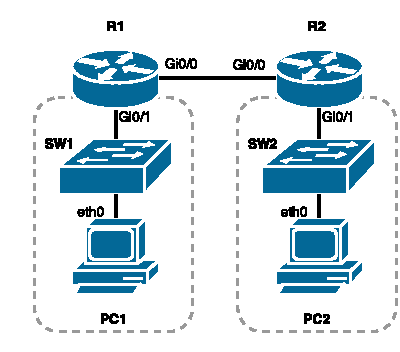
\includegraphics[width=0.6\textwidth]{figures/labtop}
                    \caption{Physical lab topology.}
                    \label{fig:labtop}
                \end{figure}

            \item Run Wireshark on all involved lab PCs as depicted in Figure
                \ref{fig:labtop}.
            \item Configure the interfaces:
                \begin{itemize}
                    \item Configure\footnote{\texttt{enable}, \texttt{configure
                        terminal}, \texttt{interface Gi0/0}, \texttt{ip address
                        10.0.0.1 255.255.255.0}.} \texttt{R1}'s interfaces as follows:
                        \begin{itemize}
                            \item GigabitEthernet 0/0: IPv4 address 10.0.12.1,
                                subnet mask 255.255.255.0.
                            \item GigabitEthernet 0/1: IPv4 address 10.0.1.1,
                                subnet mask 255.255.255.0.
                        \end{itemize}
                    \item Configure \texttt{R2}'s interfaces as follows:
                        \begin{itemize}
                            \item GigabitEthernet 0/0: IPv4 address 10.0.12.2,
                                subnet mask 255.255.255.0.
                            \item GigabitEthernet 0/1: IPv4 address 10.0.2.1,
                                subnet mask 255.255.255.0.
                        \end{itemize}
                    \item Configure\footnote{\texttt{ifconfig eth0 10.0.1.2/24}}
                        \texttt{\texttt{PC1}}'s interfaces as follows:
                        \begin{itemize}
                            \item eth0: IPv4 address 10.0.1.2,
                                subnet mask 255.255.255.0.
                        \end{itemize}
                    \item Configure \texttt{\texttt{PC2}}'s interfaces as follows:
                        \begin{itemize}
                            \item eth0: IPv4 address 10.0.2.2,
                                subnet mask 255.255.255.0.
                        \end{itemize}
                \end{itemize}
                
            \item Then add the IP routing tables as follows:
                \begin{itemize}
                    \item For R1: \texttt{ip route 10.0.2.0 255.255.255.0
                        10.0.12.2}
                    \item For R2: \texttt{ip route 10.0.1.0 255.255.255.0
                        10.0.12.1}
                    \item For PC1: \texttt{route add -net 0.0.0.0/0 gw
                        10.0.1.1}
                    \item For PC2: \texttt{route add -net 0.0.0.0/0 gw
                                10.0.2.1}
                \end{itemize}
            \item Apply the following modifications to the TCP behaviour of the
                involved PCs:
                \begin{itemize}
                    \item Disable TCP \texttt{RST}
                        messages\footnote{\texttt{iptables -A OUTPUT -p tcp
                        --tcp-flags RST RST -j DROP}}. This due to the fact
                        that you will be using raw sockets which do not
                        register connections in the kernel-maintained
                        connections table, which causes the respond with
                        \texttt{RST} packets as it thinks that there is no
                        corresponding connection for the received TCP packets.
                    \item Extend the \texttt{SYN-RECEIVED}
                        period\footnote{\texttt{sysctl -w
                        net.ipv4.tcp\_synack\_retries=9999}} on the remote
                        peer. This is simply to give you more time to figure
                        out what should the response be before the remote peer
                        decides to give up the connection and free its its
                        resources.
                \end{itemize}
            \item Test connectivity using the \texttt{ping} command to send
                ICMP Echo messages to PCs in other networks and receive the
                respective ICMP Echo-Reply messages back.
        \end{enumerate}

    \section{Lab experiments}
        \subsection{Connection establishment and data transmission}
            \begin{flushright}
                \textbf{[100 points]}\marginnote{\small \textbf{Note:} When done, show your
                work to the lab engineer for grading purposes.}
            \end{flushright}

            Using the \texttt{nc}\footnote{\texttt{nc -l -p 100 -s 10.0.1.2}}
            command run three applications on PC1 that listen on TCP ports as
            follows:
            \begin{itemize}
                \item Application 1: listen on IP 10.0.1.2 and TCP port 100.
                \item Application 2: listen on IP 10.0.1.2 and TCP port 200.
                \item Application 3: listen on IP 10.0.1.2 and TCP port 300
            \end{itemize}

            Then, using the provided tools (\texttt{macframesender.c}) send the
            following messages by using TCP:
            \begin{itemize}
                \item Message data: "Hello".
                \item Source: PC2. 
                \item Destination: to PC1's \texttt{nc} process that is
                    listening on port 100.
            \end{itemize}

            \subsubsection{Notes}
                \begin{itemize}
                    \item Appendix \ref{a} contains a description of protocol
                        formats.
                    \item Comment your \texttt{macframesender.c}. This can
                        help you identify the problems much faster.
                    \item You can save your time by organizing your code by
                        copying \texttt{macframesender.c} into multiple files
                        such as \texttt{syn.c}, \texttt{ack.c}, \texttt{psh.c}.
                        This way you can repeat previous tasks much easier
                        (except for updating the \texttt{ACK} number and TCP's
                        checksum.
                    \item The tool \texttt{nc} will not accept subsequent
                        connections from \emph{other} source IP addresses and
                        source port numbers after it is used by some source IP
                        and source port. Note that this is only a limitation in
                        \texttt{nc} and it is easy to code TCP servers that
                        accept connections from multiple clients.
                \end{itemize}

        \subsection{Connection termination (extra question; not graded)}
            Terminate the TCP connection above using the FIN 3-way hand-shake.
            

    \newpage
    \appendix
    \section{Protocol header formats and IDs}\label{a}
        Protocol IDs: IP = \texttt{0x0800}, TCP = \texttt{0x06}.
                \begin{figure}[tbh]
                    \centering
                    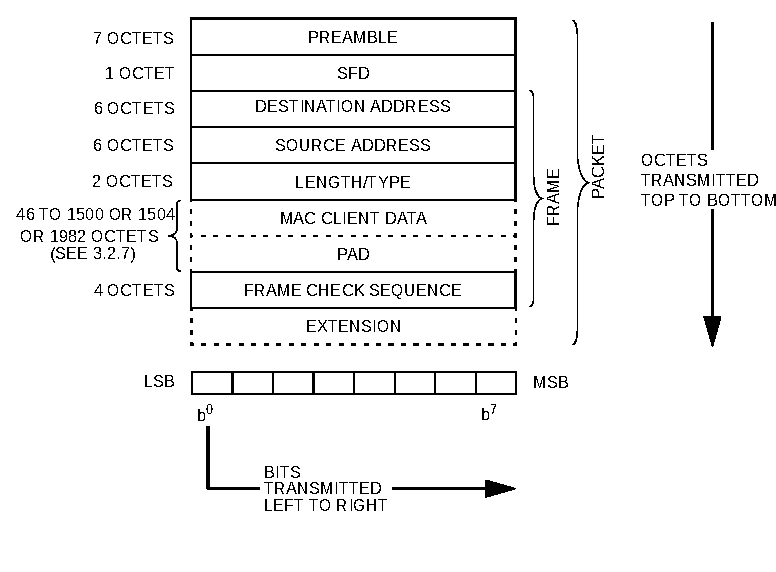
\includegraphics[width=0.9\textwidth]{figures/macpacket}
                    \vspace{-15pt}
                    \caption{Ethernet Media Access Control (MAC) packet (note
                    that an octet is 8 bits) --- Source: IEEE Std. 802.3-2012.}
                    \label{fig:macpacket}
                \end{figure}

                \begin{figure}[tbh]
                    \centering
                    \small\begin{verbatim} 0                   1                   2                   3
 0 1 2 3 4 5 6 7 8 9 0 1 2 3 4 5 6 7 8 9 0 1 2 3 4 5 6 7 8 9 0 1
+-+-+-+-+-+-+-+-+-+-+-+-+-+-+-+-+-+-+-+-+-+-+-+-+-+-+-+-+-+-+-+-+
|Version|  IHL  |Type of Service|          Total Length         |
+-+-+-+-+-+-+-+-+-+-+-+-+-+-+-+-+-+-+-+-+-+-+-+-+-+-+-+-+-+-+-+-+
|         Identification        |Flags|      Fragment Offset    |
+-+-+-+-+-+-+-+-+-+-+-+-+-+-+-+-+-+-+-+-+-+-+-+-+-+-+-+-+-+-+-+-+
|  Time to Live |    Protocol   |         Header Checksum       |
+-+-+-+-+-+-+-+-+-+-+-+-+-+-+-+-+-+-+-+-+-+-+-+-+-+-+-+-+-+-+-+-+
|                       Source Address                          |
+-+-+-+-+-+-+-+-+-+-+-+-+-+-+-+-+-+-+-+-+-+-+-+-+-+-+-+-+-+-+-+-+
|                    Destination Address                        |
+-+-+-+-+-+-+-+-+-+-+-+-+-+-+-+-+-+-+-+-+-+-+-+-+-+-+-+-+-+-+-+-+
|                    Options                    |    Padding    |
+-+-+-+-+-+-+-+-+-+-+-+-+-+-+-+-+-+-+-+-+-+-+-+-+-+-+-+-+-+-+-+-+\end{verbatim}\normalsize
                    \vspace{-15pt}
                    \caption{Internet Protocol (IP) version 4 header format --- Source RFC791.}
                    \label{fig:ipv4}
                \end{figure}


\end{document}
